% Options for packages loaded elsewhere
% Options for packages loaded elsewhere
\PassOptionsToPackage{unicode}{hyperref}
\PassOptionsToPackage{hyphens}{url}
\PassOptionsToPackage{dvipsnames,svgnames,x11names}{xcolor}
%
\documentclass[
  letterpaper,
  DIV=11,
  numbers=noendperiod]{scrartcl}
\usepackage{xcolor}
\usepackage{amsmath,amssymb}
\setcounter{secnumdepth}{-\maxdimen} % remove section numbering
\usepackage{iftex}
\ifPDFTeX
  \usepackage[T1]{fontenc}
  \usepackage[utf8]{inputenc}
  \usepackage{textcomp} % provide euro and other symbols
\else % if luatex or xetex
  \usepackage{unicode-math} % this also loads fontspec
  \defaultfontfeatures{Scale=MatchLowercase}
  \defaultfontfeatures[\rmfamily]{Ligatures=TeX,Scale=1}
\fi
\usepackage{lmodern}
\ifPDFTeX\else
  % xetex/luatex font selection
\fi
% Use upquote if available, for straight quotes in verbatim environments
\IfFileExists{upquote.sty}{\usepackage{upquote}}{}
\IfFileExists{microtype.sty}{% use microtype if available
  \usepackage[]{microtype}
  \UseMicrotypeSet[protrusion]{basicmath} % disable protrusion for tt fonts
}{}
\makeatletter
\@ifundefined{KOMAClassName}{% if non-KOMA class
  \IfFileExists{parskip.sty}{%
    \usepackage{parskip}
  }{% else
    \setlength{\parindent}{0pt}
    \setlength{\parskip}{6pt plus 2pt minus 1pt}}
}{% if KOMA class
  \KOMAoptions{parskip=half}}
\makeatother
% Make \paragraph and \subparagraph free-standing
\makeatletter
\ifx\paragraph\undefined\else
  \let\oldparagraph\paragraph
  \renewcommand{\paragraph}{
    \@ifstar
      \xxxParagraphStar
      \xxxParagraphNoStar
  }
  \newcommand{\xxxParagraphStar}[1]{\oldparagraph*{#1}\mbox{}}
  \newcommand{\xxxParagraphNoStar}[1]{\oldparagraph{#1}\mbox{}}
\fi
\ifx\subparagraph\undefined\else
  \let\oldsubparagraph\subparagraph
  \renewcommand{\subparagraph}{
    \@ifstar
      \xxxSubParagraphStar
      \xxxSubParagraphNoStar
  }
  \newcommand{\xxxSubParagraphStar}[1]{\oldsubparagraph*{#1}\mbox{}}
  \newcommand{\xxxSubParagraphNoStar}[1]{\oldsubparagraph{#1}\mbox{}}
\fi
\makeatother

\usepackage{color}
\usepackage{fancyvrb}
\newcommand{\VerbBar}{|}
\newcommand{\VERB}{\Verb[commandchars=\\\{\}]}
\DefineVerbatimEnvironment{Highlighting}{Verbatim}{commandchars=\\\{\}}
% Add ',fontsize=\small' for more characters per line
\usepackage{framed}
\definecolor{shadecolor}{RGB}{241,243,245}
\newenvironment{Shaded}{\begin{snugshade}}{\end{snugshade}}
\newcommand{\AlertTok}[1]{\textcolor[rgb]{0.68,0.00,0.00}{#1}}
\newcommand{\AnnotationTok}[1]{\textcolor[rgb]{0.37,0.37,0.37}{#1}}
\newcommand{\AttributeTok}[1]{\textcolor[rgb]{0.40,0.45,0.13}{#1}}
\newcommand{\BaseNTok}[1]{\textcolor[rgb]{0.68,0.00,0.00}{#1}}
\newcommand{\BuiltInTok}[1]{\textcolor[rgb]{0.00,0.23,0.31}{#1}}
\newcommand{\CharTok}[1]{\textcolor[rgb]{0.13,0.47,0.30}{#1}}
\newcommand{\CommentTok}[1]{\textcolor[rgb]{0.37,0.37,0.37}{#1}}
\newcommand{\CommentVarTok}[1]{\textcolor[rgb]{0.37,0.37,0.37}{\textit{#1}}}
\newcommand{\ConstantTok}[1]{\textcolor[rgb]{0.56,0.35,0.01}{#1}}
\newcommand{\ControlFlowTok}[1]{\textcolor[rgb]{0.00,0.23,0.31}{\textbf{#1}}}
\newcommand{\DataTypeTok}[1]{\textcolor[rgb]{0.68,0.00,0.00}{#1}}
\newcommand{\DecValTok}[1]{\textcolor[rgb]{0.68,0.00,0.00}{#1}}
\newcommand{\DocumentationTok}[1]{\textcolor[rgb]{0.37,0.37,0.37}{\textit{#1}}}
\newcommand{\ErrorTok}[1]{\textcolor[rgb]{0.68,0.00,0.00}{#1}}
\newcommand{\ExtensionTok}[1]{\textcolor[rgb]{0.00,0.23,0.31}{#1}}
\newcommand{\FloatTok}[1]{\textcolor[rgb]{0.68,0.00,0.00}{#1}}
\newcommand{\FunctionTok}[1]{\textcolor[rgb]{0.28,0.35,0.67}{#1}}
\newcommand{\ImportTok}[1]{\textcolor[rgb]{0.00,0.46,0.62}{#1}}
\newcommand{\InformationTok}[1]{\textcolor[rgb]{0.37,0.37,0.37}{#1}}
\newcommand{\KeywordTok}[1]{\textcolor[rgb]{0.00,0.23,0.31}{\textbf{#1}}}
\newcommand{\NormalTok}[1]{\textcolor[rgb]{0.00,0.23,0.31}{#1}}
\newcommand{\OperatorTok}[1]{\textcolor[rgb]{0.37,0.37,0.37}{#1}}
\newcommand{\OtherTok}[1]{\textcolor[rgb]{0.00,0.23,0.31}{#1}}
\newcommand{\PreprocessorTok}[1]{\textcolor[rgb]{0.68,0.00,0.00}{#1}}
\newcommand{\RegionMarkerTok}[1]{\textcolor[rgb]{0.00,0.23,0.31}{#1}}
\newcommand{\SpecialCharTok}[1]{\textcolor[rgb]{0.37,0.37,0.37}{#1}}
\newcommand{\SpecialStringTok}[1]{\textcolor[rgb]{0.13,0.47,0.30}{#1}}
\newcommand{\StringTok}[1]{\textcolor[rgb]{0.13,0.47,0.30}{#1}}
\newcommand{\VariableTok}[1]{\textcolor[rgb]{0.07,0.07,0.07}{#1}}
\newcommand{\VerbatimStringTok}[1]{\textcolor[rgb]{0.13,0.47,0.30}{#1}}
\newcommand{\WarningTok}[1]{\textcolor[rgb]{0.37,0.37,0.37}{\textit{#1}}}

\usepackage{longtable,booktabs,array}
\usepackage{calc} % for calculating minipage widths
% Correct order of tables after \paragraph or \subparagraph
\usepackage{etoolbox}
\makeatletter
\patchcmd\longtable{\par}{\if@noskipsec\mbox{}\fi\par}{}{}
\makeatother
% Allow footnotes in longtable head/foot
\IfFileExists{footnotehyper.sty}{\usepackage{footnotehyper}}{\usepackage{footnote}}
\makesavenoteenv{longtable}
\usepackage{graphicx}
\makeatletter
\newsavebox\pandoc@box
\newcommand*\pandocbounded[1]{% scales image to fit in text height/width
  \sbox\pandoc@box{#1}%
  \Gscale@div\@tempa{\textheight}{\dimexpr\ht\pandoc@box+\dp\pandoc@box\relax}%
  \Gscale@div\@tempb{\linewidth}{\wd\pandoc@box}%
  \ifdim\@tempb\p@<\@tempa\p@\let\@tempa\@tempb\fi% select the smaller of both
  \ifdim\@tempa\p@<\p@\scalebox{\@tempa}{\usebox\pandoc@box}%
  \else\usebox{\pandoc@box}%
  \fi%
}
% Set default figure placement to htbp
\def\fps@figure{htbp}
\makeatother


% definitions for citeproc citations
\NewDocumentCommand\citeproctext{}{}
\NewDocumentCommand\citeproc{mm}{%
  \begingroup\def\citeproctext{#2}\cite{#1}\endgroup}
\makeatletter
 % allow citations to break across lines
 \let\@cite@ofmt\@firstofone
 % avoid brackets around text for \cite:
 \def\@biblabel#1{}
 \def\@cite#1#2{{#1\if@tempswa , #2\fi}}
\makeatother
\newlength{\cslhangindent}
\setlength{\cslhangindent}{1.5em}
\newlength{\csllabelwidth}
\setlength{\csllabelwidth}{3em}
\newenvironment{CSLReferences}[2] % #1 hanging-indent, #2 entry-spacing
 {\begin{list}{}{%
  \setlength{\itemindent}{0pt}
  \setlength{\leftmargin}{0pt}
  \setlength{\parsep}{0pt}
  % turn on hanging indent if param 1 is 1
  \ifodd #1
   \setlength{\leftmargin}{\cslhangindent}
   \setlength{\itemindent}{-1\cslhangindent}
  \fi
  % set entry spacing
  \setlength{\itemsep}{#2\baselineskip}}}
 {\end{list}}
\usepackage{calc}
\newcommand{\CSLBlock}[1]{\hfill\break\parbox[t]{\linewidth}{\strut\ignorespaces#1\strut}}
\newcommand{\CSLLeftMargin}[1]{\parbox[t]{\csllabelwidth}{\strut#1\strut}}
\newcommand{\CSLRightInline}[1]{\parbox[t]{\linewidth - \csllabelwidth}{\strut#1\strut}}
\newcommand{\CSLIndent}[1]{\hspace{\cslhangindent}#1}



\setlength{\emergencystretch}{3em} % prevent overfull lines

\providecommand{\tightlist}{%
  \setlength{\itemsep}{0pt}\setlength{\parskip}{0pt}}



 


\usepackage{fvextra}
\DefineVerbatimEnvironment{Verbatim}{Verbatim}{breaklines=true,breakanywhere=true}
\KOMAoption{captions}{tableheading}
\makeatletter
\@ifpackageloaded{caption}{}{\usepackage{caption}}
\AtBeginDocument{%
\ifdefined\contentsname
  \renewcommand*\contentsname{Table of contents}
\else
  \newcommand\contentsname{Table of contents}
\fi
\ifdefined\listfigurename
  \renewcommand*\listfigurename{List of Figures}
\else
  \newcommand\listfigurename{List of Figures}
\fi
\ifdefined\listtablename
  \renewcommand*\listtablename{List of Tables}
\else
  \newcommand\listtablename{List of Tables}
\fi
\ifdefined\figurename
  \renewcommand*\figurename{Figure}
\else
  \newcommand\figurename{Figure}
\fi
\ifdefined\tablename
  \renewcommand*\tablename{Table}
\else
  \newcommand\tablename{Table}
\fi
}
\@ifpackageloaded{float}{}{\usepackage{float}}
\floatstyle{ruled}
\@ifundefined{c@chapter}{\newfloat{codelisting}{h}{lop}}{\newfloat{codelisting}{h}{lop}[chapter]}
\floatname{codelisting}{Listing}
\newcommand*\listoflistings{\listof{codelisting}{List of Listings}}
\makeatother
\makeatletter
\makeatother
\makeatletter
\@ifpackageloaded{caption}{}{\usepackage{caption}}
\@ifpackageloaded{subcaption}{}{\usepackage{subcaption}}
\makeatother
\usepackage{bookmark}
\IfFileExists{xurl.sty}{\usepackage{xurl}}{} % add URL line breaks if available
\urlstyle{same}
\hypersetup{
  pdftitle={Tarea 3 Transcriptómica},
  pdfauthor={Mateo Jiménez-Sotelo - LCG22},
  colorlinks=true,
  linkcolor={blue},
  filecolor={Maroon},
  citecolor={Blue},
  urlcolor={Blue},
  pdfcreator={LaTeX via pandoc}}


\title{Tarea 3 Transcriptómica}
\usepackage{etoolbox}
\makeatletter
\providecommand{\subtitle}[1]{% add subtitle to \maketitle
  \apptocmd{\@title}{\par {\large #1 \par}}{}{}
}
\makeatother
\subtitle{Nextflow}
\author{Mateo Jiménez-Sotelo - LCG22}
\date{2026-02-04}
\begin{document}
\maketitle


\begin{verbatim}
Tarea en el path:
/export/space3/users/majiso/LCG_Gen22/\ 
LCG_Sem4/Transcriptomica/Tabula_Muris_Transcriptomics_2026
\end{verbatim}

\begin{quote}
Servidor: \texttt{Chaac}
\end{quote}

\section{Introducción}\label{introducciuxf3n}

\subsection{Planteamiento}\label{planteamiento}

\emph{Nextflow} es un motor de flujo de trabajo que permite la ejecución
de \emph{pipelines} de análisis de datos de manera \textbf{reproducible}
y \textbf{escalable} (Di Tommaso et al. (2017)). Está basado en
\emph{Groovy}, un lenguaje de programación dinámico que se ejecuta sobre
la máquina virtual de \emph{Java}, lo que no solo le permite utilizar
una sintaxis similar a la de lenguajes modernos, como \emph{python},
sino que le confiere bastante flexibilidad y portabilidad (Seandavi
(2020)). \emph{Nextflow} facilita la gestión de dependencias y manejo de
versiones, así como la paralelización de tareas y la integración con
sistemas de cómputo en la nube mediante \textbf{directivas}. En
conjunto, esta herramienta es idónea para el análisis de datos genómicos
a gran escala.

Los pipelines de \emph{Nextflow} se definen en un archivo \texttt{.nf},
que contiene:

\begin{itemize}
\item
  \textbf{Funciones}: Son bloques de código auxiliares utilizados para
  lógica simple dentro del \emph{script}, como manipulación de
  \emph{strings} o parámetros, pero \textbf{no} forman parte del flujo
  de ejecución del \emph{pipeline}.
\item
  \textbf{Procesos}: Son las unidades básicas de ejecución en
  \emph{Nextflow}. Cada proceso define una tarea específica, incluyendo
  sus entradas (input), salidas (output) y el bloque de código que se
  ejecutará.
\item
  \textbf{\emph{Workflows}}: Definen cómo se conectan los procesos,
  especificando el flujo de datos entre las distintas etapas del
  \emph{pipeline} y determinando qué información se transmite y cómo lo
  hace.
\item
  \textbf{Canales}: Son las estructuras de datos que permiten la
  comunicación entre procesos, facilitando el paso de información y
  resultados de uno a otro. Estos se generan precisamente en los
  procesos o \emph{workflows} y pueden ser nombrados mediante
  \texttt{emit} para facilitar su uso.
\item
  \textbf{Directivas}: Son las configuraciones declarativas dentro de
  los procesos que especifican recursos computacionales como CPU y
  memoria, el entorno de ejecución, manejo de errores y otras
  condiciones que controlan cómo y dónde se ejecuta cada tarea.
\item
  \textbf{Contenedores}: \emph{Nextflow} permite la integración con
  sistemas de contenedores como \emph{Docker} o \emph{Singularity}, lo
  que facilita la gestión de dependencias y versiones de software,
  asegurando la reproducibilidad del análisis en distintos entornos de
  cómputo, sean locales o \emph{HPC}.
\end{itemize}

\subsection{Objetivos}\label{objetivos}

\textbf{Objetivo general}

\begin{itemize}
\tightlist
\item
  Utilizar \emph{Nextflow} para implementar un \emph{pipeline} que
  permita correr \texttt{FastQC} (Andrews (2010)) sobre los archivos
  \texttt{fastq} crudos de un directorio dado, los limpie con
  \texttt{fastp} (Chen et al. (2018)) y ejecute nuevamente
  \texttt{FastQC} sobre los archivos limpios.
\end{itemize}

\textbf{Objetivos específicos}

\begin{itemize}
\item
  Definir un \emph{pipeline} de análisis de datos genómicos utilizando
  \emph{Nextflow}.
\item
  Familiarizarse con la sintaxis y estructura de los archivos
  \texttt{.nf}.
\item
  Implementar un flujo de trabajo reproducible y escalable con
  \emph{directivas}.
\item
  Ajustar parámetros de \texttt{fastp} en función de métricas de calidad
  obtenidas previamente con \texttt{FastQC}.
\end{itemize}

\section{Metodología y
justificación}\label{metodologuxeda-y-justificaciuxf3n}

\subsection{\texorpdfstring{Sintaxis y estructura de archivos
\texttt{.nf}}{Sintaxis y estructura de archivos .nf}}\label{sintaxis-y-estructura-de-archivos-.nf}

Los \emph{pipelines} de \emph{Nextflow} se definen en un archivo con
extensión \texttt{.nf} con la siguiente estructura:

\begin{verbatim}
// Definir funciones auxiliares
def foo_func(param) {
  // Código de la función
  <...>
  return result
}

// Definir procesos
process <process_name> {
  // Generar outputs en el wd
  publishDir <'path'>
  // Archivos o variables que toma el proceso
  input:
    path <path>
  // Canales generados --> 'emit' si quieren nombrarse
  output:
    path <'foo_output_file_1'>, emit: <channel_1_name>
    <...>
    path <'foo_output_file_n'>
  // Comandos de bash propios del proceso
  script/shell:
    """
    <bash script que genere los n outputs>
    """
}

// Definir workflows --> Auxiliares con nombre, principal sin
workflow <workflow_name>{
  // Crear canal de entrada básico
  // 'fromFilePairs' para canal según archivos con un patrón dado
  reads = Channel.fromFilePairs("<pattern>")

  // Ejecución de procesos y manejo de canales
  foo = <process_name>(reads)

  // '.out' es un iterable de los outputs del proceso
  foo_func(foo.out)

  // '.<channel_name>' para identificarlo por su nombre
  foo.out.<channel_name>

  // Enlazar procesos usando canales
  bar = <process_name>(foo.out.<channel_name>)

  // Emitir canales para su uso en otros procesos o workflows
  emit:
    <channel_name> = bar.out
}
\end{verbatim}

\begin{quote}
Ejemplo general de la estructura de un archivo \texttt{.nf} con
funciones auxiliares, procesos y workflows. Se incluyen directivas,
manejo de inputs/outputs y uso de \texttt{emit} para nombrar canales. En
la práctica, la estructura puede variar según las necesidades del
análisis, pero este \emph{chunk} sirve como guía básica para organizar
el código.
\end{quote}

Adicionalmente, los \emph{pipelines} pueden modularizarse separando los
\emph{procesos} en archivos externos independientes.

\begin{quote}
Para los ambientes de conda, \emph{Nextflow} crea un entorno específico
para cada proceso y lo guarda en \emph{caché} para su uso en tanto se
ejecute el \emph{workflow}.
\end{quote}

\subsection{Estrategia}\label{estrategia}

Previamente, en la tarea 1 (\texttt{./tarea\_1.qmd}), se realizaron
análisis de calidad antes y después de la limpieza de los archivos
\texttt{fastq} con los programas \texttt{FastQC} y \texttt{MultiQC}
(Ewels et al. (2016)), y \texttt{fastp}, respectivamente.

Para el análisis de calidad, se usaron los siguientes comandos en ambas
ocasiones:

\begin{Shaded}
\begin{Highlighting}[]
\ExtensionTok{fastqc}\NormalTok{ –t 4 –o ./}\OperatorTok{\textless{}}\NormalTok{output\_dir}\OperatorTok{\textgreater{}}\NormalTok{ ./}\OperatorTok{\textless{}}\NormalTok{input\_dir}\OperatorTok{\textgreater{}}\NormalTok{/}\PreprocessorTok{*}\NormalTok{.fastq.gz}
\ExtensionTok{multiqc}\NormalTok{ ./}\OperatorTok{\textless{}}\NormalTok{out\_dir}\OperatorTok{\textgreater{}}
\end{Highlighting}
\end{Shaded}

Asimismo, la limpieza se hizo con el siguiente \emph{script}:

\begin{Shaded}
\begin{Highlighting}[]
\CommentTok{\#!/bin/bash}
\CommentTok{\#$ {-}cwd}
\CommentTok{\#$ {-}o data/trimmed/fastp\_$JOB\_ID.out}
\CommentTok{\#$ {-}e data/trimmed/fastp\_$JOB\_ID.err}

\VariableTok{RAW\_PATH}\OperatorTok{=}\StringTok{"./data/raw"}
\VariableTok{TRIMMED\_PATH}\OperatorTok{=}\StringTok{"./data/trimmed"}

\FunctionTok{mkdir} \AttributeTok{{-}p} \VariableTok{$TRIMMED\_PATH}

\VariableTok{LOG}\OperatorTok{=}\StringTok{"}\VariableTok{$\{TRIMMED\_PATH\}}\StringTok{/fastp\_log.txt"}
\BuiltInTok{echo} \StringTok{"Starting job on }\VariableTok{$(}\FunctionTok{hostname}\VariableTok{)}\StringTok{"} \OperatorTok{\textgreater{}} \VariableTok{$LOG}
\BuiltInTok{echo} \StringTok{"Date: }\VariableTok{$(}\FunctionTok{date}\VariableTok{)}\StringTok{"} \OperatorTok{\textgreater{}\textgreater{}} \VariableTok{$LOG}

\ExtensionTok{conda}\NormalTok{ activate fastp}

\ControlFlowTok{for}\NormalTok{ file }\KeywordTok{in} \VariableTok{$\{RAW\_PATH\}}\NormalTok{/SRR}\PreprocessorTok{*}\NormalTok{\_1.fastq.gz}\KeywordTok{;} \ControlFlowTok{do}
  \VariableTok{srr}\OperatorTok{=}\VariableTok{$(}\FunctionTok{basename} \StringTok{"}\VariableTok{$file}\StringTok{"}\NormalTok{ \_1.fastq.gz}\VariableTok{)} \CommentTok{\# Solo el SRR}

  \CommentTok{\# Paired End}
  \ExtensionTok{fastp} \DataTypeTok{\textbackslash{}}
    \AttributeTok{{-}i} \VariableTok{$\{RAW\_PATH\}}\NormalTok{/}\VariableTok{$\{srr\}}\NormalTok{\_1.fastq.gz }\DataTypeTok{\textbackslash{}}
    \AttributeTok{{-}I} \VariableTok{$\{RAW\_PATH\}}\NormalTok{/}\VariableTok{$\{srr\}}\NormalTok{\_2.fastq.gz }\DataTypeTok{\textbackslash{}}
    \AttributeTok{{-}o} \VariableTok{$\{TRIMMED\_PATH\}}\NormalTok{/}\VariableTok{$\{srr\}}\NormalTok{\_1.trimmed.fastq.gz }\DataTypeTok{\textbackslash{}}
    \AttributeTok{{-}O} \VariableTok{$\{TRIMMED\_PATH\}}\NormalTok{/}\VariableTok{$\{srr\}}\NormalTok{\_2.trimmed.fastq.gz }\DataTypeTok{\textbackslash{}}
    \AttributeTok{{-}{-}detect\_adapter\_for\_pe} \DataTypeTok{\textbackslash{}}
    \AttributeTok{{-}{-}trim\_poly\_g} \DataTypeTok{\textbackslash{}}
    \AttributeTok{{-}{-}cut\_tail} \DataTypeTok{\textbackslash{}}
    \AttributeTok{{-}{-}thread}\NormalTok{ 8 }\DataTypeTok{\textbackslash{}}
    \AttributeTok{{-}{-}json} \VariableTok{$\{TRIMMED\_PATH\}}\NormalTok{/}\VariableTok{$\{srr\}}\NormalTok{.json }\DataTypeTok{\textbackslash{}}
    \AttributeTok{{-}{-}html} \VariableTok{$\{TRIMMED\_PATH\}}\NormalTok{/}\VariableTok{$\{srr\}}\NormalTok{.html}
\ControlFlowTok{done}

\ExtensionTok{conda}\NormalTok{ deactivate}

\BuiltInTok{echo} \StringTok{"Job finished at }\VariableTok{$(}\FunctionTok{date}\VariableTok{)}\StringTok{"} \OperatorTok{\textgreater{}\textgreater{}} \VariableTok{$LOG}
\end{Highlighting}
\end{Shaded}

Para adaptarlo a un \emph{pipeline} de \emph{Nextflow}, se optó por
\emph{re-definir} \textbf{un proceso por tarea}. De este modo, se busca
mantener la trazabilidad de los procesos y delegar el \emph{caching} y
manejo de \emph{inputs}/\emph{outputs} a \emph{Nextflow} al tiempo que
se aprovecha la capacidad de \textbf{paralelización} del programa
\textbf{mediante los canales}.

La tarea se puede estructurar como un \emph{workflow} con dos procesos
principales, \texttt{QC} y \texttt{CLEANING}, donde \texttt{QC} se
reutiliza para evaluar tanto los datos crudos como los procesados.

\subsection{Parseo para limpieza}\label{parseo-para-limpieza}

La idea inicial era hacer un \emph{pipeline} que recibiera los
parámetros de \texttt{fastp} a modo de argumentos, pero esto se vuelve
problemático porque implica, o fragmentar el \emph{pipeline} en dos
partes a modo de \emph{checkpoint}, primero para hacer el análisis de
calidad de las lecturas crudas y luego para, con base en eso y los
argumentos dados por el usuario, ejecutar la limpieza; o bien,
proporcionar los parámetros de limpieza desde el inicio, lo que
implicaría que se conoce la calidad de las lecturas \emph{a priori}.

Así, dado que la otra opción sería usar parámetros estáticos, se optó
por implementar un proceso intermedio que, a partir del
\texttt{summary.txt} contenido en el \texttt{.zip} que genera
\texttt{FastQC}, extraiga métricas de calidad relevantes y genere un
archivo de texto por muestra con los parámetros de limpieza a usar en
\texttt{fastp}. De este modo, aunque el usuario no puede modificar los
parámetros de limpieza, estos sí se ajustan a la calidad de las lecturas
crudas. Dado que las métricas de calidad pueden variar entre muestras y
\emph{Nextflow} posibilita el procesamiento de archivos de forma
individual, se aplican correcciones únicamente cuando son necesarias,
evitando la eliminación innecesaria de información en muestras con buena
calidad y usando un criterio, si bien arbitrario, consistente,
reproducible y basado en métricas objetivas.

\subsubsection{Criterios de
corrección}\label{criterios-de-correcciuxf3n}

Se asume que los \texttt{fastq} son datos de RNA-seq de \emph{Illumina},
por lo que no se atienden secuencias sobrerepresentadas, niveles de
duplicación o contenido de \emph{GC}.

\begin{quote}
Justificación conceptual más profunda puede consultarse en la tarea 1,
sección de \textbf{Análisis de calidad} (\texttt{./tarea\_1.qmd}).
\end{quote}

Así, las únicas métricas de calidad que se consideran para ajustar las
\emph{flags} de limpieza sin \emph{sobreparametrizar} son:

\begin{quote}
Se añade el parámetro correspondiente de \texttt{fastp} si el estatus de
la métrica es \texttt{WARN} o \texttt{FAIL}.
\end{quote}

\begin{itemize}
\tightlist
\item
  \textbf{Adapter Content}: \texttt{-\/-detect\_adapter\_for\_pe}

  \begin{itemize}
  \tightlist
  \item
    Detecta y elimina adaptadores en datos \emph{PE}.
  \end{itemize}
\item
  \textbf{Per base sequence quality}: \texttt{-\/-cut\_tail}

  \begin{itemize}
  \tightlist
  \item
    Elimina bases de baja calidad al final de las lecturas.
  \end{itemize}
\end{itemize}

\subsubsection{Parser de python}\label{parser-de-python}

El \emph{script} usado es \texttt{./src/parse\_fastqc.py}:

\begin{quote}
Se usa \texttt{zipfile} para acceder al \texttt{summary.txt} del
\texttt{.zip} sin descomprimir el archivo
\end{quote}

\begin{Shaded}
\begin{Highlighting}[]
\ImportTok{import}\NormalTok{ argparse}
\ImportTok{import}\NormalTok{ zipfile}

\CommentTok{\# Argumentos}
\NormalTok{parser }\OperatorTok{=}\NormalTok{ argparse.ArgumentParser(}
\NormalTok{  description}\OperatorTok{=}\StringTok{"Return fastp parameters based on FastQC summary.txt"}
\NormalTok{)}
\NormalTok{parser.add\_argument(}
  \StringTok{"zip"}\NormalTok{,}
  \BuiltInTok{help}\OperatorTok{=}\StringTok{"FastQC .zip file containing summary.txt for a sample"}
\NormalTok{)}
\NormalTok{args }\OperatorTok{=}\NormalTok{ parser.parse\_args()}
\NormalTok{zip\_path }\OperatorTok{=}\NormalTok{ args.}\BuiltInTok{zip}

\CommentTok{\# Leer summary.txt}
\NormalTok{flags }\OperatorTok{=} \BuiltInTok{set}\NormalTok{() }\CommentTok{\# Set para evitar duplicar parámetros}
\NormalTok{might\_use }\OperatorTok{=}\NormalTok{ [}\StringTok{"FAIL"}\NormalTok{, }\StringTok{"WARN"}\NormalTok{]}

\CommentTok{\# Abrir el archivo zip}
\ControlFlowTok{with}\NormalTok{ zipfile.ZipFile(zip\_path, }\StringTok{\textquotesingle{}r\textquotesingle{}}\NormalTok{) }\ImportTok{as}\NormalTok{ zip\_file:}
  \CommentTok{\# Encontrar summary.txt dentro del zip}
\NormalTok{  summary\_file }\OperatorTok{=}\NormalTok{ [}
    \BuiltInTok{file} \ControlFlowTok{for} \BuiltInTok{file} \KeywordTok{in}\NormalTok{ zip\_file.namelist() }\ControlFlowTok{if} \BuiltInTok{file}\NormalTok{.endswith(}\StringTok{"summary.txt"}\NormalTok{)}
\NormalTok{    ][}\DecValTok{0}\NormalTok{]}

  \CommentTok{\# Leer summary.txt línea por línea}
  \ControlFlowTok{with}\NormalTok{ zip\_file.}\BuiltInTok{open}\NormalTok{(summary\_file) }\ImportTok{as} \BuiltInTok{file}\NormalTok{:}
    \ControlFlowTok{for}\NormalTok{ line }\KeywordTok{in} \BuiltInTok{file}\NormalTok{:}
\NormalTok{      line }\OperatorTok{=}\NormalTok{ line.decode().strip()}
      \CommentTok{\# Estatus por cada estadística}
\NormalTok{      status, statistic, \_ }\OperatorTok{=}\NormalTok{ line.split(}\StringTok{"}\CharTok{\textbackslash{}t}\StringTok{"}\NormalTok{)}

      \CommentTok{\# Correspondencia fastqc{-}fastp}
      \ControlFlowTok{if}\NormalTok{ statistic }\OperatorTok{==} \StringTok{"Adapter Content"} \KeywordTok{and}\NormalTok{ status }\KeywordTok{in}\NormalTok{ might\_use:}
\NormalTok{        flags.add(}\StringTok{"{-}{-}detect\_adapter\_for\_pe"}\NormalTok{)}

      \ControlFlowTok{if}\NormalTok{ statistic }\OperatorTok{==} \StringTok{"Per base sequence quality"} \KeywordTok{and}\NormalTok{ status }\KeywordTok{in}\NormalTok{ might\_use:}
\NormalTok{        flags.add(}\StringTok{"{-}{-}cut\_tail"}\NormalTok{)}

\CommentTok{\# Siempre, asumiendo datos de Illumina}
\NormalTok{flags.add(}\StringTok{"{-}{-}trim\_poly\_g"}\NormalTok{)}

\CommentTok{\# Output {-}{-}\textgreater{} flags separadas por espacio}
\BuiltInTok{print}\NormalTok{(}\StringTok{" "}\NormalTok{.join(}\BuiltInTok{sorted}\NormalTok{(flags)).strip())}
\end{Highlighting}
\end{Shaded}

\subsection{Pipeline}\label{pipeline}

El flujo inicia con la creación de un canal de entrada a partir de los
archivos fastq, los cuales se agrupan automáticamente por muestra,
permitiendo distinguir entre datos single-end y paired-end según el
número de archivos asociados. A partir de este canal, los procesos se
encadenan mediante el paso explícito de sus salidas
(\texttt{.out}/\textless{}\texttt{nombre\ dado\ en\ emit}\textgreater)
como entradas del siguiente paso. Los resultados de \texttt{FastQC} son
posteriormente procesados mediante el script auxiliar de
\texttt{python}, que extrae métricas de calidad y genera parámetros de
entrada para fastp, permitiendo así una limpieza \emph{semi-dinámica} de
las lecturas. Finalmente, \texttt{emit} se utiliza para exponer los
resultados relevantes del \emph{workflow} para su inspección o uso
posterior.

\subsubsection{Módulos}\label{muxf3dulos}

El uso de módulos en \emph{Nextflow} permite organizar el código de
manera más limpia y reutilizable. En este caso, se separan los procesos
\texttt{FASTQC}, \texttt{PARSE\_QC}, \texttt{FASTP} y \texttt{MULTIQC}
en archivos \texttt{.nf} independientes y se importan en el archivo
principal. Esto no solo facilita la mantenibilidad del código, sino que
permite reutilizar procesos durante el \emph{pipeline}.

\begin{quote}
DSL2 no permite isntanciar un proceso dos veces dentro del mismo
\emph{workflow}, por lo que más bien se importa desde un módulo bajo dos
nombres diferentes.
\end{quote}

\begin{quote}
Aunque \texttt{fastqc}, \texttt{fastp} y \texttt{python} están
disponibles en el entorno base de \emph{Chaac}, se especifican entornos
de conda con las versiones específicas de los programas disponibles por
\emph{default} en el servidor para cada proceso, asegurando
reproducibilidad.
\end{quote}

\paragraph{FastQC}\label{fastqc}

\texttt{./src/fastqc.nf}:

\begin{verbatim}
// FastQC
process FASTQC {
  conda "bioconda::fastqc=0.12.1"

  input:
    val stage
    // Agrupar por muestra
    tuple val(sample_id), path(reads)

  // Mode copy para no mover los archivos originales
  publishDir "${params.outdir}/fastqc_${stage}", mode: 'copy'

  output:
    // El .zip de FastQC es el input para el proceso de parseo
    tuple val(sample_id), path("*.zip"), emit: zip

  script:
    // FastQC a todas las reads, separadas por espacio
    """
    fastqc -t 4 ${reads.join(' ')}
    """
}
\end{verbatim}

\paragraph{Parseo de parámetros}\label{parseo-de-paruxe1metros}

\texttt{./src/parse\_fastqc.nf}:

\begin{verbatim}
// Parseo de resultados de FastQC --> Parámetros de fastp
process PARSE_QC {
  conda "conda-forge::python=3.9"
  input:
    tuple val(sample_id), path(qc_zip)
    path parse_script

  output:
    tuple val(sample_id), path("${sample_id}.params.txt"), emit: params

  // Script auxiliar de python para parámetros dinámicos
  script:
    """
    python ${parse_script} ${qc_zip} > \
    ${sample_id}.params.txt
    """
}
\end{verbatim}

\paragraph{Limpieza con fastp}\label{limpieza-con-fastp}

\texttt{./src/fastp.nf}:

\begin{verbatim}
// Limpieza con fastp --> SE + PE
process FASTP {
  conda "bioconda::fastp=0.24.1"
  publishDir "${params.outdir}/trimmed", mode: 'copy'

  input:
    tuple val(sample_id), path(reads), path(param_file)

  output:
    tuple val(sample_id), path("*.trimmed.fastq.gz"), emit: reads
    path "${sample_id}.json", emit: json
    path "${sample_id}.html", emit: html

  script:
    // PE o SE según número de archivos asociados a la muestra
    def is_paired = reads.size() == 2

    def input_args = is_paired ?
      "-i ${reads[0]} -I ${reads[1]}" : "-i ${reads[0]}"

    def output_args = is_paired ?
      "-o ${sample_id}_1.trimmed.fastq.gz -O ${sample_id}_2.trimmed.fastq.gz" :
      "-o ${sample_id}.trimmed.fastq.gz"

    """
    fastp \
    ${input_args} \
    ${output_args} \
    \$(cat ${param_file}) \
    --thread 4 \
    --json ${sample_id}.json \
    --html ${sample_id}.html
    """
}
\end{verbatim}

\paragraph{MultiQC}\label{multiqc}

\texttt{./src/multiqc.nf}:

\begin{verbatim}
/ Calidad general
process MULTIQC {
  conda "bioconda::multiqc=1.33"

  input:
    val stage
    path qc_files

  publishDir "${params.outdir}/multiqc_${stage}", mode: 'copy'

  output:
    path "multiqc_report.html"

  script:
    """
    multiqc ${qc_files} -o .
    """
}
\end{verbatim}

\subsubsection{Workflow}\label{workflow}

El \emph{script} del \emph{workflow} del \emph{pipeline} es
\texttt{./src/nextflow\_QC\_cleaning.nf}:

\begin{verbatim}
#!/usr/bin/env nextflow
nextflow.enable.dsl=2

// Módulos

include { FASTQC as FASTQC_RAW } from './fastqc.nf'
include { FASTQC as FASTQC_CLEAN } from './fastqc.nf'
include { PARSE_QC } from './parse_fastqc.nf'
include { FASTP } from './fastp.nf'
include { MULTIQC as MULTIQC_RAW } from './multiqc.nf'
include { MULTIQC as MULTIQC_CLEAN } from './multiqc.nf'

// Parámetros

// Input y output con valores por defecto
params.input = params.input ?: "./data/raw/*.fastq.gz"
params.outdir = params.outdir ?: "./results/nextflow"


// Workflow

workflow {
  // Canal de entrada --> PE o SE dinámicamente
  // Tupla (sample id, reads) --> Agrupado por sample id
  reads = Channel
    .fromPath(params.input, checkIfExists: true)
    .map { file ->
      def sample = file.baseName.replaceAll(/_[12]$/, "")
      tuple(sample, file)
    }
    .groupTuple()

  // FastQC inicial
  qc_raw = FASTQC_RAW("raw", reads)

  // MultiQC --> Recolecta todos los .zip de FastQC
  multiqc_raw = MULTIQC_RAW(
    "raw",
    qc_raw.zip.map { it[1] }.collect()
  )

  // Parseo de métricas → parámetros dinámicos
  parsed = PARSE_QC(qc_raw.zip, file("./src/parse_fastqc.py"))

  // Asociar params con cada muestra
  reads_with_params = reads.join(parsed)

  // Limpieza con fastp
  trimmed = FASTP(reads_with_params)

  // FastQC final
  qc_clean = FASTQC_CLEAN("clean", trimmed.reads)

  // MultiQC final
  multiqc_clean = MULTIQC_CLEAN(
    "clean",
    qc_clean.zip.map { it[1] }.collect()
  )
}
\end{verbatim}

\begin{quote}
El \emph{pipeline} asume que los nombres de los archivos \texttt{fastq}
siguen el formato \texttt{SRR*\_1.fastq.gz} y \texttt{SRR*\_2.fastq.gz}
para datos \emph{PE} y \texttt{*.fastq.gz} para \emph{SE}.
\end{quote}

\subsection{Pruebas}\label{pruebas}

\subsubsection{Paired-end}\label{paired-end}

Para correr el pipeline, se usa el siguiente comando:

\begin{quote}
El input usa un patrón que incluye todos los archivos del directorio,
por lo que el pipeline procesa \emph{paired-end}.
\end{quote}

\begin{Shaded}
\begin{Highlighting}[]
\ExtensionTok{nextflow}\NormalTok{ run ./src/nextflow\_QC\_cleaning.nf }\DataTypeTok{\textbackslash{}}
  \AttributeTok{{-}{-}input} \StringTok{"./data/raw/*.fastq.gz"} \DataTypeTok{\textbackslash{}}
  \AttributeTok{{-}{-}outdir} \StringTok{"./results/nextflow\_PE"} \DataTypeTok{\textbackslash{}}
  \AttributeTok{{-}with{-}conda} \DataTypeTok{\textbackslash{}}
  \AttributeTok{{-}with{-}report}\NormalTok{ report\_PE.html }\DataTypeTok{\textbackslash{}}
  \AttributeTok{{-}with{-}trace}\NormalTok{ trace\_PE.txt }\DataTypeTok{\textbackslash{}}
  \AttributeTok{{-}with{-}timeline}\NormalTok{ timeline\_PE.html}
\end{Highlighting}
\end{Shaded}

Y se obtiene:

\begin{verbatim}
 N E X T F L O W   ~  version 24.04.3

Launching `./src/nextflow_QC_cleaning.nf` [stupefied_rosalind] DSL2 - revision: 54e9cd60d5

executor >  local (66)
[92/68699f] process > FASTQC_RAW (12)   [100%] 16 of 16 ✔
[1c/f2ba57] process > MULTIQC_RAW       [100%] 1 of 1 ✔
[19/b25c9d] process > PARSE_QC (16)     [100%] 16 of 16 ✔
[ed/aff68d] process > FASTP (16)        [100%] 16 of 16 ✔
[84/1a0527] process > FASTQC_CLEAN (16) [100%] 16 of 16 ✔
[36/99a260] process > MULTIQC_CLEAN     [100%] 1 of 1 ✔
Completed at: 01-May-2026 21:50:09
Duration    : 7m 14s
CPU hours   : 1.5
Succeeded   : 66
\end{verbatim}

Constatamos que los archivos de salida sean los esperados:

\begin{Shaded}
\begin{Highlighting}[]
\FunctionTok{ls}\NormalTok{ ./results/nextflow\_PE }\KeywordTok{\&\&} \DataTypeTok{\textbackslash{}}
\FunctionTok{ls}\NormalTok{ ./results/nextflow\_PE/fastqc\_raw }\KeywordTok{|} \FunctionTok{wc} \AttributeTok{{-}l} \KeywordTok{\&\&} \DataTypeTok{\textbackslash{}}
\FunctionTok{ls}\NormalTok{ ./results/nextflow\_PE/fastqc\_clean }\KeywordTok{|} \FunctionTok{wc} \AttributeTok{{-}l} \KeywordTok{\&\&} \DataTypeTok{\textbackslash{}}
\FunctionTok{ls}\NormalTok{ ./results/nextflow\_PE/trimmed/}\PreprocessorTok{*}\NormalTok{fastq.gz }\KeywordTok{|} \FunctionTok{wc} \AttributeTok{{-}l} \KeywordTok{\&\&} \DataTypeTok{\textbackslash{}}
\FunctionTok{ls}\NormalTok{ ./results/nextflow\_PE/multiqc\_}\PreprocessorTok{*}
\end{Highlighting}
\end{Shaded}

\begin{verbatim}
fastqc_clean
fastqc_raw
multiqc_clean
multiqc_raw
trimmed
16
16
16
./results/nextflow_PE/multiqc_clean:
multiqc_report.html

./results/nextflow_PE/multiqc_raw:
multiqc_report.html
\end{verbatim}

\subsubsection{Single-end}\label{single-end}

Para correr el pipeline, se usa el siguiente comando:

\begin{quote}
El input incluye solo los archivos \texttt{*\_1.fastq.gz}, por lo que el
pipeline procesa \emph{single-end}.
\end{quote}

\begin{quote}
Dado que el pipeline ya se ejecutó con los archivos \emph{PE} y los
procesos están \emph{cacheados}, se añade \texttt{-resume} para evitar
la re-ejecución de los procesos que ya tuvieran sus outputs generados,
en aras de una ejecución más rápida.
\end{quote}

\begin{Shaded}
\begin{Highlighting}[]
\ExtensionTok{nextflow}\NormalTok{ run ./src/nextflow\_QC\_cleaning.nf }\DataTypeTok{\textbackslash{}}
  \AttributeTok{{-}{-}input} \StringTok{"./data/raw/*\_1.fastq.gz"} \DataTypeTok{\textbackslash{}}
  \AttributeTok{{-}{-}outdir} \StringTok{"./results/nextflow\_SE"} \DataTypeTok{\textbackslash{}}
  \AttributeTok{{-}with{-}conda} \DataTypeTok{\textbackslash{}}
  \AttributeTok{{-}with{-}report}\NormalTok{ report\_SE.html }\DataTypeTok{\textbackslash{}}
  \AttributeTok{{-}with{-}trace}\NormalTok{ trace\_SE.txt }\DataTypeTok{\textbackslash{}}
  \AttributeTok{{-}with{-}timeline}\NormalTok{ timeline\_SE.html }\DataTypeTok{\textbackslash{}}
  \AttributeTok{{-}resume}
\end{Highlighting}
\end{Shaded}

Y se obtiene:

\begin{verbatim}
 N E X T F L O W   ~  version 24.04.3

Launching `./src/nextflow_QC_cleaning.nf` [boring_cray] DSL2 - revision: 54e9cd60d5

executor >  local (2)
[08/2f0a14] process > FASTQC_RAW (6)   [100%] 8 of 8, cached: 8 ✔
[6d/704b48] process > MULTIQC_RAW      [100%] 1 of 1 ✔
[eb/8ab0bf] process > PARSE_QC (5)     [100%] 8 of 8, cached: 8 ✔
[5f/a4f5ef] process > FASTP (2)        [100%] 8 of 8, cached: 8 ✔
[9f/da269a] process > FASTQC_CLEAN (8) [100%] 8 of 8, cached: 8 ✔
[6e/79ad24] process > MULTIQC_CLEAN    [100%] 1 of 1 ✔
\end{verbatim}

Constatamos que los archivos de salida sean los esperados:

\begin{Shaded}
\begin{Highlighting}[]
\FunctionTok{ls}\NormalTok{ ./results/nextflow\_SE }\KeywordTok{\&\&} \DataTypeTok{\textbackslash{}}
\FunctionTok{ls}\NormalTok{ ./results/nextflow\_SE/fastqc\_raw }\KeywordTok{|} \FunctionTok{wc} \AttributeTok{{-}l} \KeywordTok{\&\&} \DataTypeTok{\textbackslash{}}
\FunctionTok{ls}\NormalTok{ ./results/nextflow\_SE/fastqc\_clean }\KeywordTok{|} \FunctionTok{wc} \AttributeTok{{-}l} \KeywordTok{\&\&} \DataTypeTok{\textbackslash{}}
\FunctionTok{ls}\NormalTok{ ./results/nextflow\_SE/trimmed/}\PreprocessorTok{*}\NormalTok{fastq.gz }\KeywordTok{|} \FunctionTok{wc} \AttributeTok{{-}l} \KeywordTok{\&\&} \DataTypeTok{\textbackslash{}}
\FunctionTok{ls}\NormalTok{ ./results/nextflow\_SE/multiqc\_}\PreprocessorTok{*}
\end{Highlighting}
\end{Shaded}

\begin{verbatim}
fastqc_clean
fastqc_raw
multiqc_clean
multiqc_raw
trimmed
8
8
8
./results/nextflow_SE/multiqc_clean:
multiqc_report.html

./results/nextflow_SE/multiqc_raw:
multiqc_report.html
\end{verbatim}

\subsection{Resultados}\label{resultados}

\begin{quote}
Para efectos de la tarea, se muestran los resultados de la ejecución con
datos \emph{paired-end}.
\end{quote}

\begin{figure}[H]

{\centering \pandocbounded{\includegraphics[keepaspectratio]{./data/images/multiqc_report_raw.png}}

}

\caption{Heatmap general del MultiQC de los archivos crudos paired-end,
procesados de forma manual en la Tarea 1}

\end{figure}%

\begin{figure}[H]

{\centering \pandocbounded{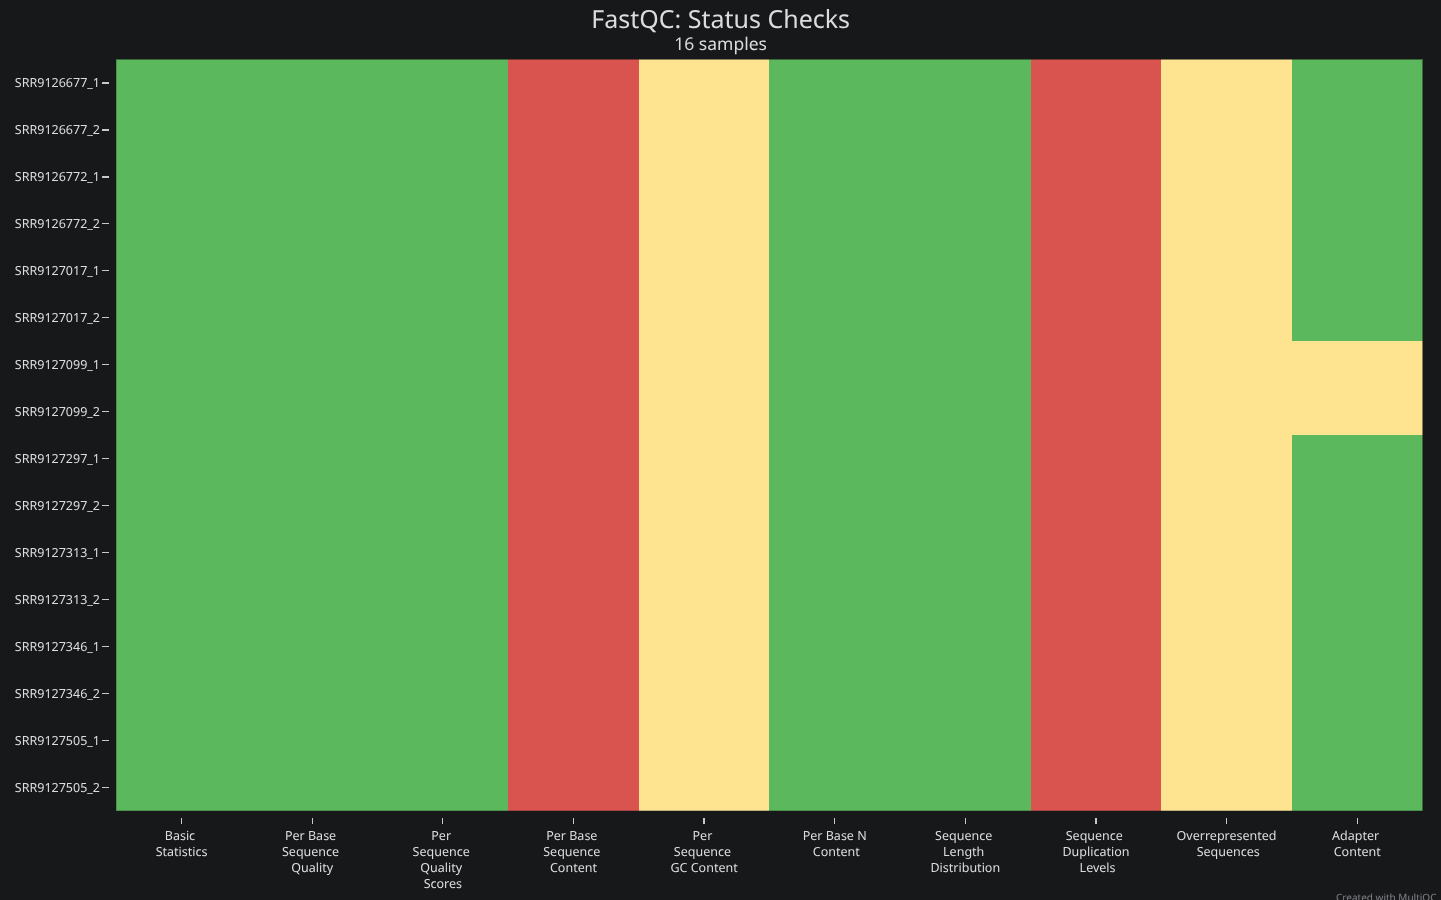
\includegraphics[keepaspectratio]{./data/images/multiqc_report_raw_nextflow.png}}

}

\caption{Heatmap general del MultiQC de los archivos crudos paired-end,
procesados mediante el pipeline de Nextflow}

\end{figure}%

\begin{figure}[H]

{\centering \pandocbounded{\includegraphics[keepaspectratio]{./data/images/multiqc_report_clean.png}}

}

\caption{Heatmap general del MultiQC de los archivos limpios paired-end,
procesados de forma manual en la Tarea 1}

\end{figure}%

\begin{figure}[H]

{\centering \pandocbounded{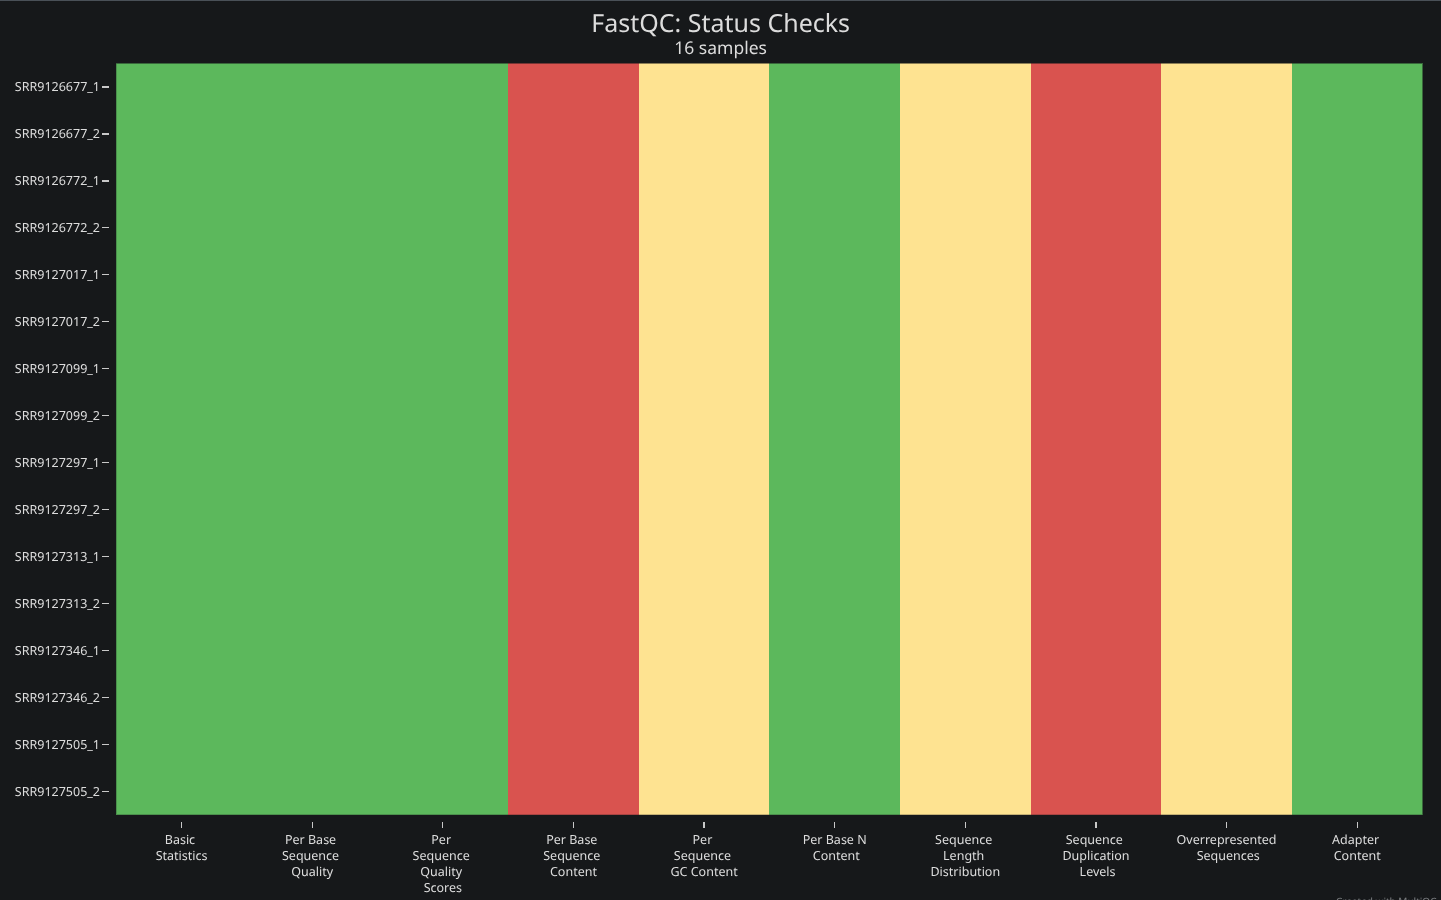
\includegraphics[keepaspectratio]{./data/images/multiqc_report_clean_nextflow.png}}

}

\caption{Heatmap general del MultiQC de los archivos limpios paired-end,
procesados mediante el pipeline de Nextflow}

\end{figure}%

\begin{center}\rule{0.5\linewidth}{0.5pt}\end{center}

\begin{figure}[H]

{\centering \pandocbounded{\includegraphics[keepaspectratio]{./data/images/adapter_content_raw.png}}

}

\caption{Contenido de adaptadores del MultiQC de los archivos crudos
paired-end, procesados de forma manual en la Tarea 1}

\end{figure}%

\begin{figure}[H]

{\centering \pandocbounded{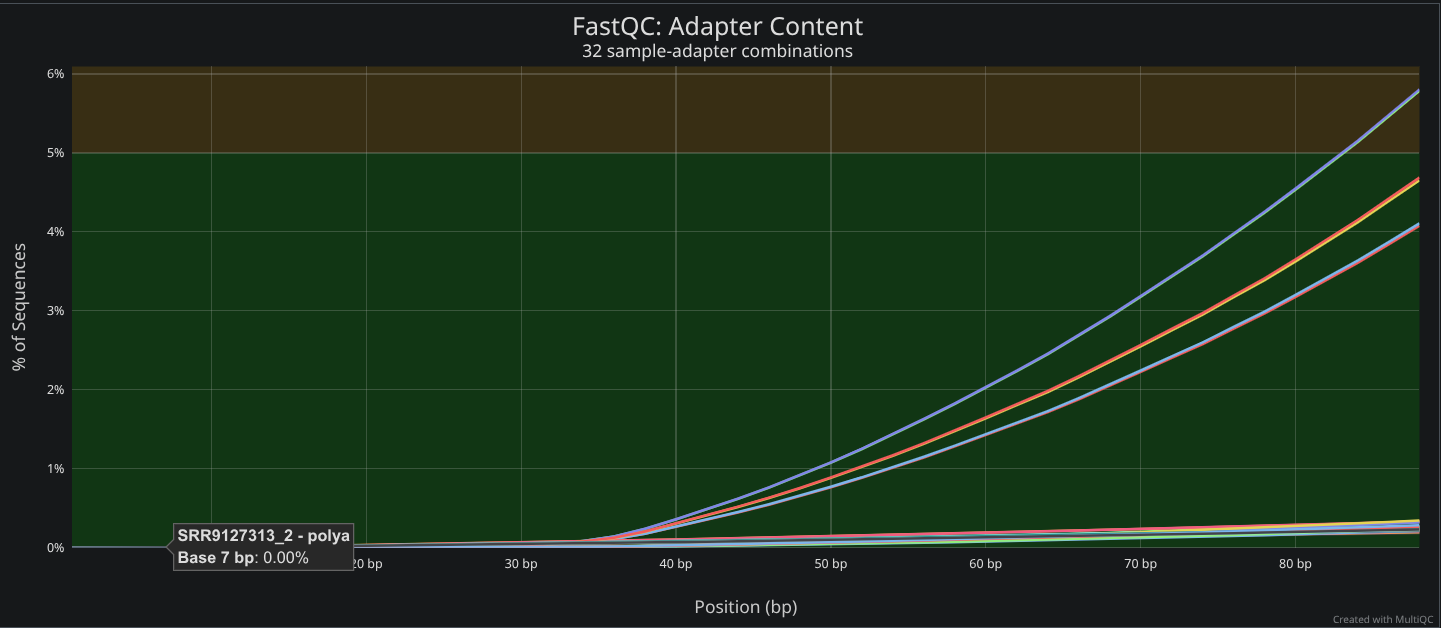
\includegraphics[keepaspectratio]{./data/images/adapter_content_raw_nextflow.png}}

}

\caption{Contenido de adaptadores del MultiQC de los archivos crudos
paired-end, procesados mediante el pipeline de Nextflow}

\end{figure}%

\begin{figure}[H]

{\centering \pandocbounded{\includegraphics[keepaspectratio]{./data/images/adapter_content_clean.png}}

}

\caption{Contenido de adaptadores del MultiQC de los archivos limpios
paired-end, procesados de forma manual en la Tarea 1}

\end{figure}%

\begin{figure}[H]

{\centering \pandocbounded{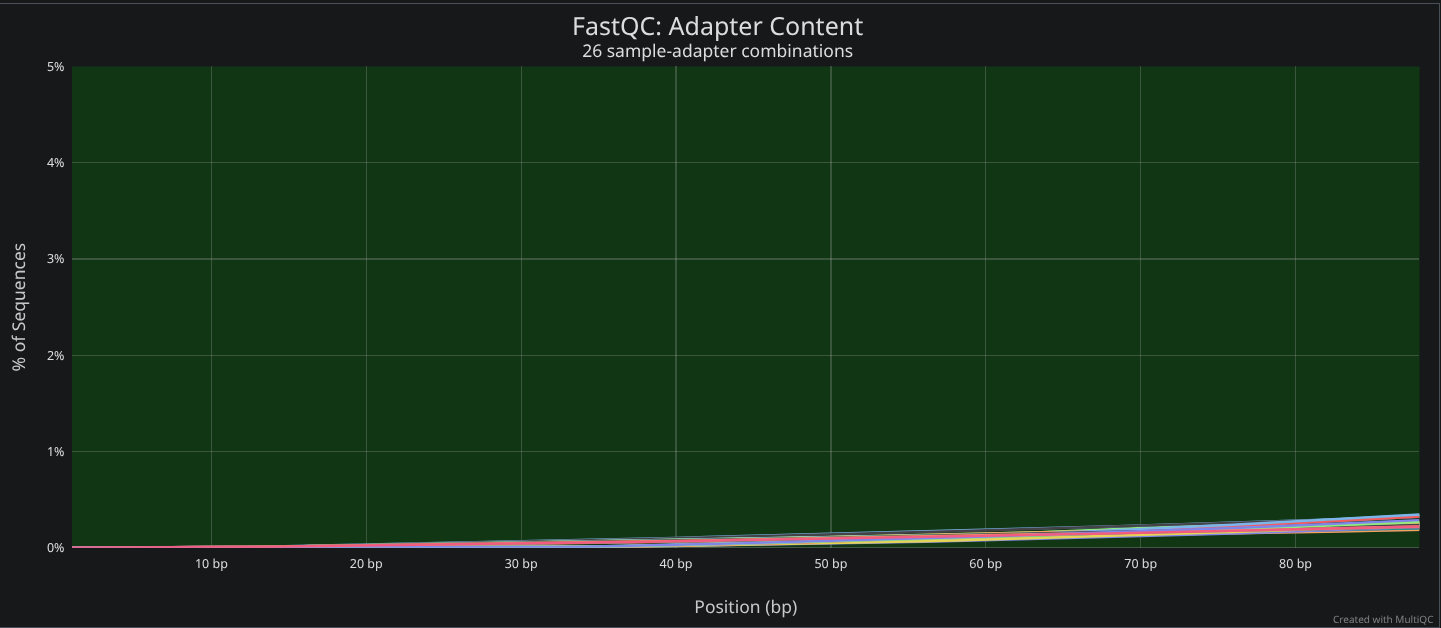
\includegraphics[keepaspectratio]{./data/images/adapter_content_clean_nextflow.png}}

}

\caption{Contenido de adaptadores del MultiQC de los archivos limpios
paired-end, procesados mediante el pipeline de Nextflow}

\end{figure}%

\section{Discusión}\label{discusiuxf3n}

Se observa que los resultados obtenidos con el \emph{pipeline} de
\emph{Nextflow} son consistentes con los de la tarea 1, indicando que la
implementación del \emph{pipeline} es correcta, coherente y
reproducible. Asimismo y acorde a la \textbf{Tarea 1}
(\texttt{./tarea\_1.qmd}), las métricas de calidad antes y después de la
limpieza muestran mejoras en el contenido de adaptadores, así como las
mismas tendencias en los demás estadísticos, lo que indica que el
proceso de limpieza se está aplicando de manera efectiva y consistente.

En términos generales y con base en los resultados obtenidos, puede
decirse que \emph{Nextflow} es una gran herramienta para homogenizar y
automatizar distintos \emph{pipelines}, facilitando su reproducibilidad
y escalabilidad en distintos entornos de cómputo, lo que es
especialmente relevante en el análisis de datos a gran escala, como lo
son los transcriptómicos; La modularización del código mediante procesos
y workflows permite una mayor flexibilidad y ofrece opciones para
reutilizar el código, mientras que el manejo de dependencias y versiones
mediante contenedores asegura la reproducibilidad del análisis.

En cuanto a tiempos de ejecución, por el output del pipeline \emph{SE},
observamos que se reutilizó toda la información previamente obtenida, a
excepción de los procesos de \texttt{MultiQC}, los cuales se ejecutaron
nuevamente para generar reportes específicos de los archivos \emph{SE}.
El primer proceso, con \emph{PE}, tardó 7 minutos con 14 segundos para
los 66 procesos individuales. Un aspecto interesante es que, pese a no
tener el registro preciso del tiempo de ejecución del segundo proceso,
es inmediatamente notorio que \emph{Nextflow} y su capacidad de
paralelización mediante canales permite una ejecución del pipeline muy
veloz, siempre y cuando -como en este caso- se hayan \emph{cacheado} ya
los procesos y ambientes internos, lo que ofrece una ventaja en los
análisis a gran escala.

Por los \texttt{./trace\_*.txt}, podemos determinar cuánto tardó cada
proceso individualmente:

\begin{quote}
\texttt{./trace\_PE.txt}
\end{quote}

Si tomamos en cuenta los proceso ya realizados de cara al segundo
\emph{pipeline} en muestras \emph{SE}, notamos que, efectivamente, toda
la información se reutilizó. Así, el tiempo práctico de ejecución
refiere a los procesos \texttt{MULTIQC\_RAW} y \texttt{MULTIQC\_CLEAN}:

\begin{verbatim}
task_id hash    native_id   name    status  exit    submit  duration    realtime    %cpu    peak_rss    peak_vmem   rchar   wchar
8   c0/2bcfc4   3863339 FASTQC_RAW (15) CACHED  0   2026-05-01 21:42:56.434 1m 51s  1m 50s  101.9%  1.3 GB  5.6 GB  972.6 MB    1.8 MB
1   8f/168539   3863318 FASTQC_RAW (1)  CACHED  0   2026-05-01 21:42:56.424 2m 21s  2m 20s  100.8%  1.3 GB  5.6 GB  1.2 GB  1.8 MB
5   b5/ecd3dd   3863235 FASTQC_RAW (9)  CACHED  0   2026-05-01 21:42:56.388 1m 30s  1m 29s  101.7%  1.4 GB  5.8 GB  751.3 MB    1.8 MB
7   cf/f99095   3863216 FASTQC_RAW (13) CACHED  0   2026-05-01 21:42:56.370 1m 54s  1m 53s  101.4%  1.3 GB  5.8 GB  1014.8 MB   1.8 MB
4   2c/604baf   3863212 FASTQC_RAW (7)  CACHED  0   2026-05-01 21:42:56.360 2m 52s  2m 51s  99.8%   1.3 GB  5.8 GB  1.4 GB  1.8 MB
3   4c/1e2cfe   3863326 FASTQC_RAW (5)  CACHED  0   2026-05-01 21:42:56.430 2m 4s   2m 3s   101.2%  1.3 GB  5.6 GB  1 GB    1.8 MB
2   47/76de20   3863253 FASTQC_RAW (3)  CACHED  0   2026-05-01 21:42:56.397 2m 44s  2m 43s  99.6%   1.3 GB  5.6 GB  1.2 GB  1.8 MB
6   08/2f0a14   3863268 FASTQC_RAW (11) CACHED  0   2026-05-01 21:42:56.406 2m 51s  2m 50s  100.8%  1.4 GB  5.8 GB  1.4 GB  1.7 MB
14  82/21bea4   3893503 PARSE_QC (3)    CACHED  0   2026-05-01 21:44:47.100 918ms   72ms    108.7%  0   0   1.1 MB  1.2 KB
10  9e/b11405   3912525 PARSE_QC (15)   CACHED  0   2026-05-01 21:45:48.052 948ms   74ms    101.5%  3.6 MB  217.5 MB    1.1 MB  1.2 KB
12  80/8c996e   3909988 PARSE_QC (12)   CACHED  0   2026-05-01 21:45:40.116 860ms   57ms    106.4%  0   0   1.1 MB  1.2 KB
15  48/e12694   3903764 PARSE_QC (9)    CACHED  0   2026-05-01 21:45:17.068 900ms   57ms    119.8%  0   0   1.1 MB  1.2 KB
11  81/9ae700   3888474 PARSE_QC (2)    CACHED  0   2026-05-01 21:44:26.117 1.1s    240ms   42.8%   13 MB   441.7 MB    1.1 MB  1.2 KB
9   76/ad8efe   3894250 PARSE_QC (5)    CACHED  0   2026-05-01 21:44:50.118 853ms   70ms    90.2%   0   0   1.1 MB  1.2 KB
16  79/1f8b1c   3897849 PARSE_QC (7)    CACHED  0   2026-05-01 21:45:00.087 930ms   66ms    102.9%  0   0   1.1 MB  1.2 KB
13  eb/8ab0bf   3912024 PARSE_QC (14)   CACHED  0   2026-05-01 21:45:47.049 956ms   80ms    102.6%  3.7 MB  217.5 MB    1.1 MB  1.2 KB
24  9b/ea9c29   3903990 FASTP (9)   CACHED  0   2026-05-01 21:45:17.985 1m 15s  1m 14s  280.2%  1.2 GB  1.8 GB  1.2 GB  1.2 GB
25  91/cf171c   3910213 FASTP (12)  CACHED  0   2026-05-01 21:45:40.996 1m 20s  1m 19s  273.2%  1.2 GB  1.9 GB  1.2 GB  1.3 GB
20  85/004b24   3898654 FASTP (7)   CACHED  0   2026-05-01 21:45:01.037 1m 1s   59.9s   400.9%  1.3 GB  1.8 GB  1 GB    1.1 GB
17  b3/4f0f74   3913067 FASTP (15)  CACHED  0   2026-05-01 21:45:49.028 1m 22s  1m 21s  368.8%  1.3 GB  1.9 GB  1.4 GB  1.5 GB
22  86/b2e35e   3888752 FASTP (1)   CACHED  0   2026-05-01 21:44:27.206 41.9s   41.1s   385.6%  1.3 GB  1.8 GB  757.3 MB    790.2 MB
19  aa/11af1a   3893673 FASTP (3)   CACHED  0   2026-05-01 21:44:48.043 59.5s   58.7s   275.9%  1.2 GB  1.8 GB  982.7 MB    1019.2 MB
21  b2/4e8173   3894994 FASTP (5)   CACHED  0   2026-05-01 21:44:50.998 1m 4s   1m 3s   298.3%  1.2 GB  1.8 GB  1 GB    1 GB
18  5f/a4f5ef   3912508 FASTP (14)  CACHED  0   2026-05-01 21:45:48.024 1m 27s  1m 26s  294.6%  1.2 GB  1.8 GB  1.4 GB  1.5 GB
26  00/d42a46   3933998 FASTQC_CLEAN (12)   CACHED  0   2026-05-01 21:47:00.829 2m 20s  2m 19s  101.4%  1.3 GB  5.7 GB  1.3 GB  1.8 MB
27  5f/eaffab   3916127 FASTQC_CLEAN (5)    CACHED  0   2026-05-01 21:45:54.753 2m 8s   2m 7s   102.0%  1.3 GB  5.8 GB  1 GB    1.8 MB
29  9c/fed5ed   3927384 FASTQC_CLEAN (9)    CACHED  0   2026-05-01 21:46:32.677 2m 32s  2m 31s  101.2%  1.4 GB  5.7 GB  1.2 GB  1.8 MB
31  2a/5094b3   3936310 FASTQC_CLEAN (14)   CACHED  0   2026-05-01 21:47:10.915 2m 39s  2m 38s  101.6%  1.3 GB  5.7 GB  1.5 GB  1.8 MB
30  4d/671b08   3900876 FASTQC_CLEAN (1)    CACHED  0   2026-05-01 21:45:09.092 1m 41s  1m 40s  102.8%  1.3 GB  5.8 GB  800.3 MB    1.8 MB
28  6c/5b0e7a   3912202 FASTQC_CLEAN (3)    CACHED  0   2026-05-01 21:45:47.569 2m 1s   2m  102.5%  1.3 GB  5.8 GB  1 GB    1.8 MB
32  62/9e4c64   3919724 FASTQC_CLEAN (7)    CACHED  0   2026-05-01 21:46:01.791 2m 12s  2m 11s  101.4%  1.3 GB  5.7 GB  1.1 GB  1.8 MB
33  9f/da269a   3937521 FASTQC_CLEAN (15)   CACHED  0   2026-05-01 21:47:15.371 2m 38s  2m 37s  101.3%  1.3 GB  5.7 GB  1.5 GB  1.8 MB
34  6e/79ad24   3999689 MULTIQC_CLEAN   COMPLETED   0   2026-05-01 22:25:38.006 8.4s    7.6s    146.2%  522.5 MB    22.5 GB 38 MB   6.3 MB
23  6d/704b48   3999683 MULTIQC_RAW COMPLETED   0   2026-05-01 22:25:37.996 8.9s    8s  121.9%  138.5 MB    13.6 GB 38 MB   6.3 MB
\end{verbatim}

Estos procesos corrieron de forma paralela y demoraron 8.4 y 8.9
segundos, respectivamente..

\section{Conclusiones}\label{conclusiones}

El \emph{pipeline} de \emph{Nextflow} implementado cumple con los
objetivos planteados, permitiendo la ejecución reproducible y escalable
de las tareas de análisis de calidad y limpieza, así como de muchos
otros anális de datos, genómicos o no. Además, la modularización del
código mediante procesos y workflows facilita su mantenimiento y
reutilización en futuros proyectos. De cara al \emph{pipeline} hecho,
los resultados obtenidos son consistentes con los análisis realizados de
forma manual en la Tarea 1 (\texttt{./tarea\_1.qmd}), validando la
correcta implementación del mismo, así como su capacidad para mejorar la
calidad de las lecturas mediante la aplicación de los parámetros de
limpieza definidos, basados en métricas objetivas extraídas de los
reportes de \texttt{FastQC}.

\section*{Referencias}\label{referencias}
\addcontentsline{toc}{section}{Referencias}

\phantomsection\label{refs}
\begin{CSLReferences}{1}{0}
\bibitem[\citeproctext]{ref-fastqc}
Andrews, S. (2010). \emph{FastQC: A quality control tool for high
throughput sequence data}.
\url{http://www.bioinformatics.babraham.ac.uk/projects/fastqc}

\bibitem[\citeproctext]{ref-10.1093ux2fbioinformaticsux2fbty560}
Chen, S., Zhou, Y., Chen, Y., \& Gu, J. (2018). Fastp: An ultra-fast
all-in-one FASTQ preprocessor. \emph{Bioinformatics}, \emph{34}(17),
i884--i890. \url{https://doi.org/10.1093/bioinformatics/bty560}

\bibitem[\citeproctext]{ref-di-tommaso-2017}
Di Tommaso, P., Chatzou, M., Floden, E. W., Barja, P. P., Palumbo, E.,
\& Notredame, C. (2017). {Nextflow enables reproducible computational
workflows}. \emph{Nature Biotechnology}, \emph{35}(4), 316--319.
\url{https://doi.org/10.1038/nbt.3820}

\bibitem[\citeproctext]{ref-Ewels_2016}
Ewels, P., Magnusson, M., Lundin, S., \& Käller, M. (2016). MultiQC:
Summarize analysis results for multiple tools and samples in a single
report. \emph{Bioinformatics}, \emph{32}(19), 3047--3048.
\url{https://doi.org/10.1093/bioinformatics/btw354}

\bibitem[\citeproctext]{ref-seandavi-2020}
Seandavi. (2020). \emph{{GitHub - seandavi/nextflow\_on\_jupyter: A
lightweight introduction to NextFlow, a workflow description language
and engine for (mainly) bioinformatics workflows. Leverages notebooks
for easy teaching.}}
\url{https://github.com/seandavi/nextflow_on_jupyter}

\end{CSLReferences}




\end{document}
